\chapter{World Model and Scenario Description}
\label{chap:worldScenModel}
The scenario in this experiment consists of simulated worlds containing UAVs, moving targets, fixed targets, and target safe havens.  The UAVs work as a team to find all the targets and destroy them.  The simulated worlds are randomly generated via a custom utility for the project.  The number of UAVs, targets, and havens are configurable.  The worlds are rectangular and their sizes are configurable.  The utility reads the configuration file and generates data files describing random worlds.  

%  See ~\ref{sec:exampleWorldCfg} for an example configuration file.

The direction of travel for moving targets is constrained to a randomly generated road network within the world.  ``Target safe havens'' are locations in world where a target may flee to and be safe from UAV attack and surveillance.  These havens are randomly located within the world on the road network.  Moving targets will travel from one haven to the next.

An example rendering of a random world is shown in figure~\ref{fig:sample_world}. Static targets are shown as red buildings.  Mobile targets are red triangles along the road.  Blue triangles are UAVs.  The yellow boxes are havens for the mobile targets.



%\end{multicols*}

\begin{figure}[H]
	\centering
	%\includegraphics[width=\linewidth,height=\textheight]{imagefile}
	%	\includegraphics[scale=0.5]{destroyed.png}
	%	\includegraphics[width=5in,height=4in,keepaspectratio=false]{destroyed.png}
	%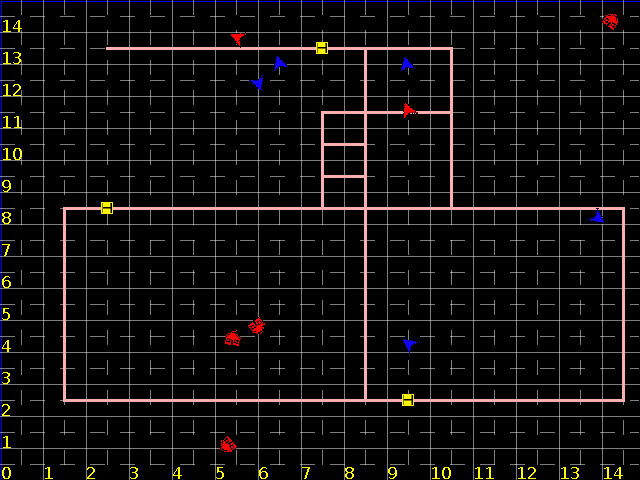
\includegraphics[width=\linewidth,height=4in,keepaspectratio=false]{world02.png}	
	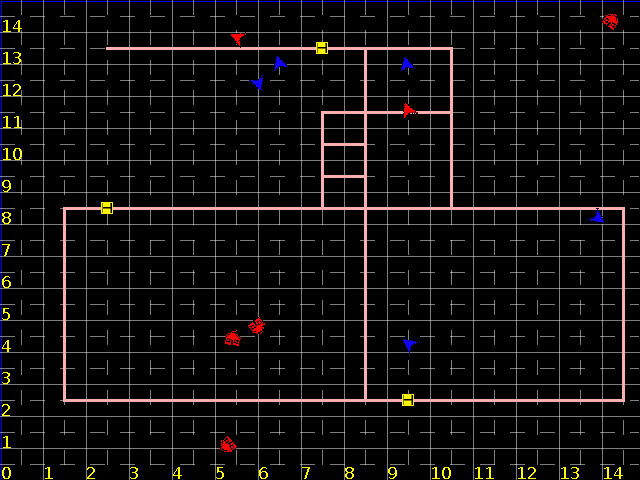
\includegraphics[scale=0.375]{world02.png}
	\caption{Sample simulated world}
	\label{fig:sample_world}
\end{figure}

%\begin{multicols*}{2}